%        File: graph_partition.tex
%     Created: Sun Mar 05 08:00 PM 2017 C
% Last Change: Sun Mar 05 08:00 PM 2017 C
%

\documentclass{beamer}
%\usetheme{Boadilla}
\usetheme{Madrid}

\title{Power Diagrams and Additively Weighted Voronoi Diagrams}
\institute{University of Minnesota}
\date{April 26, 2017}
\author{Trevor Steil}

\mode<presentation>{}

\setbeamertemplate{navigation symbols}{}

%\usepackage{amsmath}
%\usepackage{amsthm}
%\usepackage{amssymb}
%\usepackage{esint}
%\usepackage{enumitem}
\usepackage[plain]{algorithm}
\usepackage{algorithmic}
%\usepackage{algorithmicx}
%\usepackage{algpseudocode}
%\usepackage{bbm}
%\usepackage{xcolor}
\usepackage{graphicx}
\usepackage{tikz}
\usetikzlibrary{decorations.pathreplacing}
\usepackage{caption}
\usepackage[T1]{fontenc}
\usepackage[ansinew]{inputenc}
\usepackage{biblatex}
\addbibresource{project.bib}

%\newtheorem{theorem}{Theorem}[section]
%\newtheorem{corollary}{Corollary}[section]
%\newtheorem{proposition}{Proposition}[section]
%\newtheorem{lemma}{Lemma}[section]
%\newtheorem*{claim}{Claim}
%%\newtheorem*{problem}{Problem}
%%\newtheorem*{lemma}{Lemma}
%\newtheorem{definition}{Definition}[section]
%
\newcommand{\R}{\mathbb{R}}
\newcommand{\N}{\mathbb{N}}
\newcommand{\C}{\mathbb{C}}
\newcommand{\Z}{\mathbb{Z}}
\newcommand{\Q}{\mathbb{Q}}
\newcommand{\E}{\mathbb{E}}
\newcommand{\supp}[1]{\mathop{\mathrm{supp}}\left(#1\right)}
\newcommand{\lip}[1]{\mathop{\mathrm{Lip}}\left(#1\right)}
\newcommand{\curl}{\mathrm{curl}}
\newcommand{\la}{\left \langle}
\newcommand{\ra}{\right \rangle}
\renewcommand{\vec}[1]{\mathbf{#1}}
\renewcommand{\div}{\mathrm{div}}
%
%\newenvironment{problem}{\textbf{Problem.}}
%
%\newenvironment{solution}[1][]{\emph{Solution #1}}
%
%\algnewcommand{\Or}{\textbf{ or }}
%\algnewcommand{\And}{\textbf{ or }}

\setbeamertemplate{bibliography entry title}{}
\setbeamertemplate{bibliography entry location}{}
\setbeamertemplate{bibliography entry note}{}
\setbeamertemplate{bibliography item}{\insertbiblabel}


\let\Tiny=\tiny

\begin{document}

\begin{frame}
  \titlepage
\end{frame}

\begin{frame}
  \frametitle{Table of Contents}
  \tableofcontents
\end{frame}

\section{Introduction}
\begin{frame}
  \frametitle{Voronoi Diagrams}

  Given sites $S = \{ p_1, \cdots, p_n \}$, define cells
  \[ Vor(p) := \{ x \ | \ d(x,p) < d(x,q) \text{ for all } q \neq p \in S \} \]

  Generalizations:
  \begin{itemize}
    \item Order $k$ Voronoi diagram: cells share $k$ nearest sites
    \item Use different distance functions
  \end{itemize}

  We consider the second generalization through the use of weighted distances.
\end{frame}

\begin{frame}
  \frametitle{Notation}

  Throughout we will use
  \begin{itemize}
    \item Set of $n$ sites $S = \{p_1,\cdots, p_n\} \subset \R^2$
    \item Weights: $w(p)$ for all $p \in S$
  \end{itemize}

\end{frame}

\begin{frame}
  \frametitle{Multiplicatively Weighted Voronoi Diagrams}

  Define cells by
  \[ Vor_{mul}(p) = \left \{ x \ \big| \ \frac{d(x,p)}{w(p)} < \frac{d(x,q)}{w(q)} \text{ for all } q \neq p \in S \right \} \]


\end{frame}

\begin{frame}
  \frametitle{Multiplicatively Weighted Voronoi Diagrams}

  Qualitatively different than unweighted Voronoi diagram:
  \begin{itemize}
    \item Cells bounded by circular arcs
    \item Cells can be disconnected
    \item Number of connected components can be $\Theta(n^2)$
  \end{itemize}

  \begin{figure}
    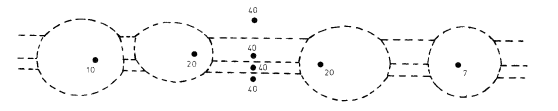
\includegraphics[width=4in]{mul(aur_surv).png}
    \caption{\footnotesize Multiplicatively Weighted Voronoi Diagram (from \cite{aurenhammer_survey})}
  \end{figure}

\end{frame}

\begin{frame}
  \frametitle{Additively Weighted Voronoi Diagrams}

  Define cells by
  \[ Vor_{add}(p) = \{ x | d(x,p) - w(p) < d(x,q) - w(q) \text{ for all } q \neq p \in S \} \]

  \begin{itemize}
    \item Have $O(n)$ faces and edges
    \item Cells bounded by hyperbolic arcs
  \end{itemize}

  \begin{figure}
    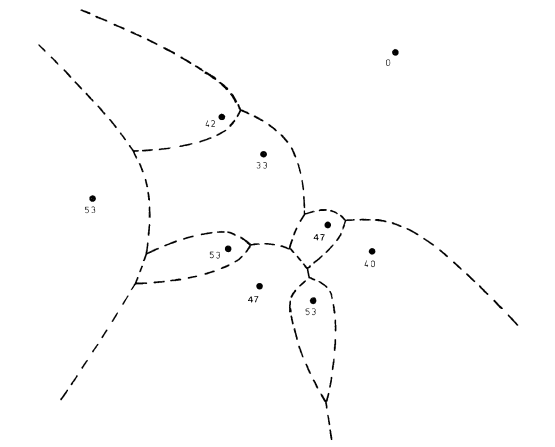
\includegraphics[width=2in]{weighted(aur_surv).png}
    \caption{Additively Weighted Voronoi Diagram (from \cite{aurenhammer_survey})}
  \end{figure}

\end{frame}

\begin{frame}
  \frametitle{Power Diagrams}

  Define power cells by
  \[ Vor_{pow}(p) = \{ x | d^2(x,p) - w^2(p) < d(x,q) - w^2(q) \text{ for all } q \neq p \in S \} \]

  \begin{itemize}
    \item Have $O(n)$ faces and edges
    \item Cells are bounded by straight lines and line segments
  \end{itemize}

  \begin{figure}
    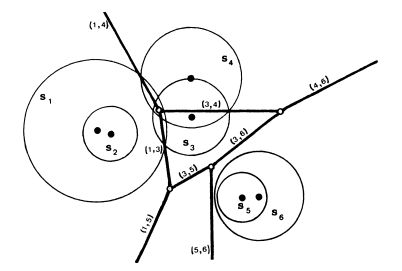
\includegraphics[width=2.5in]{power(aur_pow).png}
    \caption{Power Diagram (from \cite{aurenhammer_power})}
  \end{figure}

\end{frame}

\begin{frame}
  \frametitle{Geometric Reformulations}

  \begin{figure}
    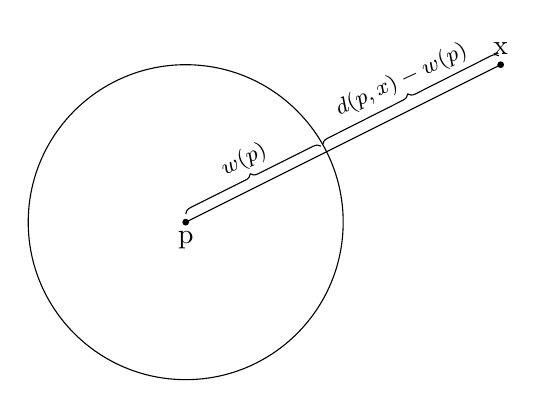
\begin{tikzpicture}
      \filldraw (0,0) circle (1pt) node(p) [align=left,below] {p} --
      (4,2) circle (1pt) node(x) [align=right,above] {x};
      \draw (0,0) circle (2);

      \draw [decorate,decoration={brace}, yshift=3pt] (0,0) -- (1.72, 0.86) node [midway, rotate=25, yshift=8pt]{\footnotesize $w(p)$};
      \draw [decorate,decoration={brace}, yshift=3pt] (1.74, 0.88) -- (3.98, 2.01) node [midway, rotate=25, yshift=8pt]{\footnotesize $d(p,x) - w(p)$};

    \end{tikzpicture}

  \end{figure}

  For additively weighted Voronoi diagrams, we can measure distances as the minimum distance to any point on a circle centered at $p$ with radius
  $w(p)$ \cite{rosenberger_additive}

\end{frame}

\begin{frame}
  \frametitle{Geometric Reformulations}

  \begin{figure}
    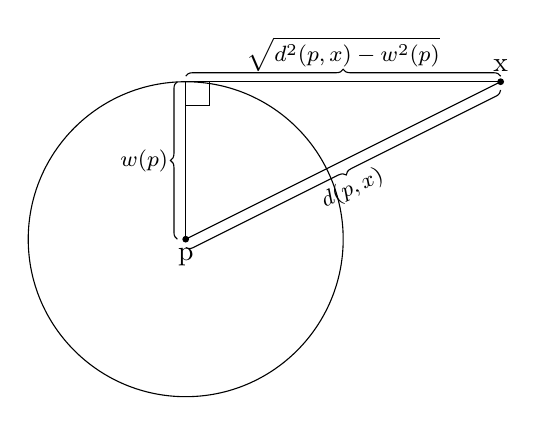
\begin{tikzpicture}

      \filldraw (0,0) circle (1pt) node(p) [align=left,below] {p} --
      (4,2) circle (1pt) node(x) [align=right,above] {x};
      \draw (0,0) circle (2);
      \draw (0,0) -- (0, 2);
      \draw (0, 2) -- (4,2);

      %Perp
      \draw (0.3, 2) -- (0.3, 1.7) -- (0, 1.7);

      \draw [decorate,decoration={brace}, xshift=-3pt] (0,0) -- (0,2) node [midway, xshift=-12pt] {\footnotesize $w(p)$};
      \draw [decorate,decoration={brace,mirror}, yshift=-3pt] (0,0) -- (4,2) node [midway, rotate=25, yshift=-8pt] {\footnotesize $d(p,x)$};
      \draw [decorate,decoration={brace}, yshift=2pt] (0,2) -- (4,2) node [midway, yshift=8pt] {\footnotesize $\sqrt{d^2(p,x) - w^2(p)}$};

    \end{tikzpicture}
  \end{figure}

  For power diagrams, we can measure distances along tangent lines to circles centered at $p$ with radius $w(p)$

\end{frame}

\begin{frame}
  \frametitle{Geometric Reformulations}

  The previous slides let us consider $S = \{ p_i \}$ as a set of sites with weights $\{ w(p_i) \}$ equivalently as a set of circles with radii $\{
  w(p_i) \}$ where we measure distances to these circles as outlined.

\end{frame}

\section{Relations to Geometric Objects in $\R^3$}
\begin{frame}
  \frametitle{Cone Arrangements and Weighted Voronoi Diagrams}

  For a site $p \in S$,
  \[ cone_p = \{ (x,y,z) \ | \ z = d(p, (x,y)) - w(p) \} \]

  \vspace{1cm}

  $Vor_{pow}(p)$ corresponds to the region of the plane $\{ z = 0 \}$ where the height of $cone_p$ is lower than $cone_q$ for all $q \neq p \in S$
  \cite{rosenberger_additive}

\end{frame}

\begin{frame}
  \frametitle{Convex Hulls and Power Diagrams}

  For a circle centered at $p = (p_x, p_y) \in S$,
  \[ \Pi(p): z = 2 p_x x + 2 p_y y - (p_x^2 + p_y^2) + w^2(p) \]

  \begin{figure}
    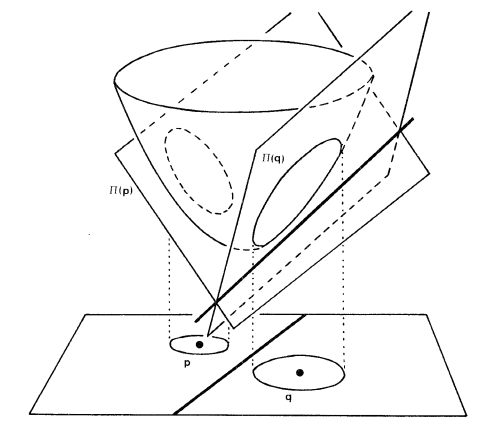
\includegraphics[width=2in]{lifting(aur_surv).png}
    \caption{Lifting map (from \cite{aurenhammer_survey})}
  \end{figure}

\end{frame}

\begin{frame}
  \frametitle{Convex Hulls and Power Diagrams}

  \begin{itemize}
    \item maps circles in $\R^2$ to nonvertical planes in $\R^3$.
    \item is a bijection between circles and nonvertical planes (that lie above the origin) \cite{aurenhammer_power}
  \end{itemize}

  For Voronoi diagrams, this same map allows phrasing Voronoi diagrams as upper envelopes of planes. \cite{comp_geom}

\end{frame}

\begin{frame}
  \frametitle{Convex Hulls and Power Diagrams}

  \begin{itemize}
    \item projecting upper envelope of $\{ \Pi(p) \ | \ p \in S \}$ gives the power diagram of $S$
    \item $\Pi$ being bijective now allows a corresponding power diagram to be found for any upper envelope of planes
    \item by duality this correspondence extends to lower convex hulls \cite{aurenhammer_power}
  \end{itemize}

\end{frame}

\begin{frame}
  \frametitle{Recognition Problems}

  When is a given diagram a power diagram or weighted Voronoi diagram?

  \vspace{1cm}

  Answer: If we know a ``reasonable'' set of sites exists and the edges are the right shape, we can find weights to fit the given diagram.

\end{frame}

\begin{frame}
  \frametitle{Power Diagram Recognition}

  Power diagram observations:
  \begin{enumerate}
    \item Power cells are convex
    \item Edges are straight and meet at vertices at angles strictly less than $\pi$ radians
    \item Edges are perpendicular to lines between sites
  \end{enumerate}

  If a given diagram satisfies 1 and 2 and a set of sites exists such that 3 is true, then weights can be found such that the power diagram matches
  the given diagram \cite{ash-bolker}

\end{frame}

\begin{frame}
  \frametitle{Power Diagram Recognition Proof Sketch}

  Idea: Look locally at a single vertex and patch together the larger diagram.

  \begin{enumerate}
    \item For a diagram with 3 edges that meet in a single vertex, show weights can be found that are consistent.
    \item On more complicated diagram, walk along edges and solve for weights as you go. By local result, weights will be compatible at every step.
  \end{enumerate}

  \begin{figure}
    \begin{tikzpicture}
      \filldraw[dashed] (0,0) circle (2pt) -- (2,2) circle (2pt) -- (3,-1) circle (2pt) -- (0,0);

      \draw (5/2, -1/2) -- (8/2, 0/2);
      \draw (5/2, -1/2) -- (4/2, -4/2);
      \draw (5/2, -1/2) -- (-1/2, 5/2);
    \end{tikzpicture}
    \caption{With appropriate sites, consistent weights can be found}
  \end{figure}

\end{frame}

\begin{frame}
  \frametitle{Weighted Voronoi Diagram Recognition}

  Weighted Voronoi diagram observations:
  \begin{enumerate}
    \item Edges are hyperbolic arcs
    \item All hyperbolas bounding a cell have a common focus (the site for the cell)
  \end{enumerate}

  If a diagram is given such that 1 is true and sites can be found to satisfy 2, the diagram coincides with a weighted Voronoi diagram
  \cite{ash-bolker}

\end{frame}

\section{Algorithms}

\begin{frame}
  \frametitle{Computing Weighted Voronoi Diagrams}

  Fortune's algorithm \cite{fortune_sweepline} \cite{rosenberger_additive}
  \begin{itemize}
    \item Sweepline algorithm (with ``beach line'')
    \item Runs in $O(n \log n)$ time
  \end{itemize}

  \begin{figure}
    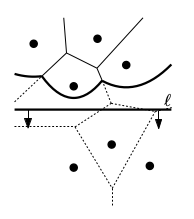
\includegraphics[width=1.5in]{beach(comp_geom).png}
    \caption{Sweepline and beach line (from \cite{comp_geom})}
  \end{figure}

\end{frame}

\begin{frame}
  \frametitle{Computing Power Diagrams}

  Method 1 \cite{aurenhammer_power} :
  \begin{itemize}
    \item Use lifting and duality to translate to convex hull problem
    \item Compute convex hull of points in $\R^3$
    \item Map convex hull back to power diagram
  \end{itemize}

  Method 2 \cite{imai_power} :
  \begin{itemize}
    \item Divide-and-conquer method of computing Voronoi diagrams also works
  \end{itemize}

  \vspace{.5cm}

  Both are $O(n \log n)$ algorithms

\end{frame}

\section{Applications}

\begin{frame}
  \frametitle{Geometric Problems with Discs}

  Let $B = \{b_1, \ldots, b_n\}$ be a set of open balls with centers $S = \{p_1, \ldots, p_n\}$

  \begin{lemma}
    \hspace{1cm} $x \in \cup_i b_i \Leftrightarrow x \in Vor_{pow}(p_i) \cap b_i$ for some $i$ \cite{aurenhammer_discs}
  \end{lemma}

  \begin{figure}
    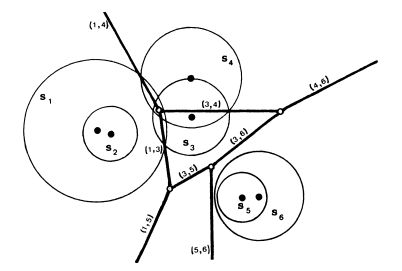
\includegraphics[width=2in]{power(aur_pow).png}
    \caption{Power diagram (from \cite{aurenhammer_power})}
  \end{figure}

\end{frame}

\begin{frame}
  \frametitle{Union of Balls Stabbing Query}

  Does a point $q$ lie in $\cup_i b_i$?

  By lemma, if and only if $q \in Vor_{pow}(p_i) \cap b_i$ for some $i$.

  \vspace{.5cm}
  Solution:
  \begin{itemize}
    \item Preprocess: build power diagram from $B$
    \item Planar point location to determine power cell $q$ lies in
    \item Check if $q$ lies in ball associated to that cell
  \end{itemize}

  Query time is $O( \log n)$.

  Can report all balls containing $q$ using colored intersections \cite{ravi}

\end{frame}

\begin{frame}
  \frametitle{Detecting Intersection of Balls}

  Do any of the balls in $B$ intersect?

  \begin{lemma}
    $b_i \cap b_j \neq \emptyset$ for some $i \neq j \Leftrightarrow b_j \cap (Vor_{pow}(p_j))^c$ for some $j$
  \end{lemma}

  Solution:
  \begin{itemize}
    \item Check each ball for containment in its own power cell
    \item $O(n \log n)$
  \end{itemize}

\end{frame}

\begin{frame}
  \frametitle{Clustering}

  Want to partition $S = \{p_1,\ldots, p_n\}$ into $S_1, \ldots, S_k$. Let $q_1, \ldots, q_k$ be associated centroids.

  \begin{theorem}
    Let $(S_1, \ldots, S_k)$ be a clustering that minimizes
    \[ \sum_{i=1}^k \sum_{p \in S_i} \| p - q_i \|^2 .\]
    By building the Voronoi diagram on $q_1, \ldots, q_k$, $S_j = S \cap Vor(q_j)$ \cite{inaba_clustering}.
  \end{theorem}

  Similarly, multiplicatively and additively weighted Voronoi diagrams can be used to minimize
  \[ \sum_{i=1}^k \frac{1}{|S_i|} \sum_{p \in S_i} \| p - q_i \|^2 .\]

\end{frame}

\begin{frame}
  \frametitle{More Applications}

  Applications continue being found:
  \begin{itemize}
    \item Cell boundaries in tissues \cite{cell}
    \item Material interfaces in fluid simulations \cite{fluids}
    \item Constrained clustering used to redistribute farmland in Germany \cite{brieden_clustering} \cite{brieden_farmland}
  \end{itemize}

  \begin{figure}
    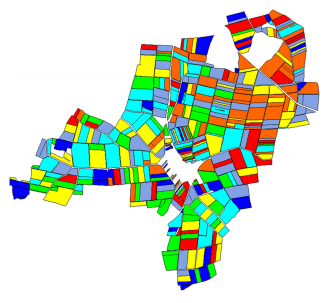
\includegraphics[width=1.5in]{farm1.png}
    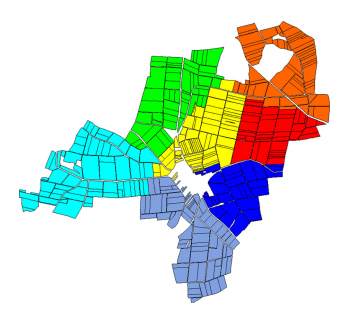
\includegraphics[width=1.5in]{farm2.png}
    \caption{Farmland redistribution (from \cite{brieden_farmland})}
  \end{figure}

\end{frame}

\begin{frame}[allowframebreaks]
  \frametitle{References}

  {\footnotesize
  \printbibliography}

\end{frame}

\end{document}


